\section{Benchmarks}
% \addcontentsline{toc}{section}{Benchmarks}

\subsection{Single-core, multi-core}
% \addcontentsline{toc}{subsection}{Single-core, multi-core}

    \paragraph*{}
    In this section, we will explore the results of restricting CPU usage to a defined number of threads, comparing 
    the performance of single-core versus multi-core execution. Ideally, one might expect a near doubling in performance 
    when the number of threads is doubled, as the workload is theoretically spread across more processing units. However, 
    in practice, the scaling is far from perfect. Various factors such as overhead from managing threads, memory access 
    bottlenecks, or CPU architecture limitations can prevent the linear scaling we might anticipate. This experiment 
    demonstrates these real-world constraints by showing the actual performance improvement as the number of threads increases.
    \par

    \vspace*{0.5cm}

    \lstinputlisting[language=Julia]{code/2-singlecore_vs_multicore/n_threads.jl}

    \begin{figure}[h]
        \begin{center}
            % Recommended preamble:
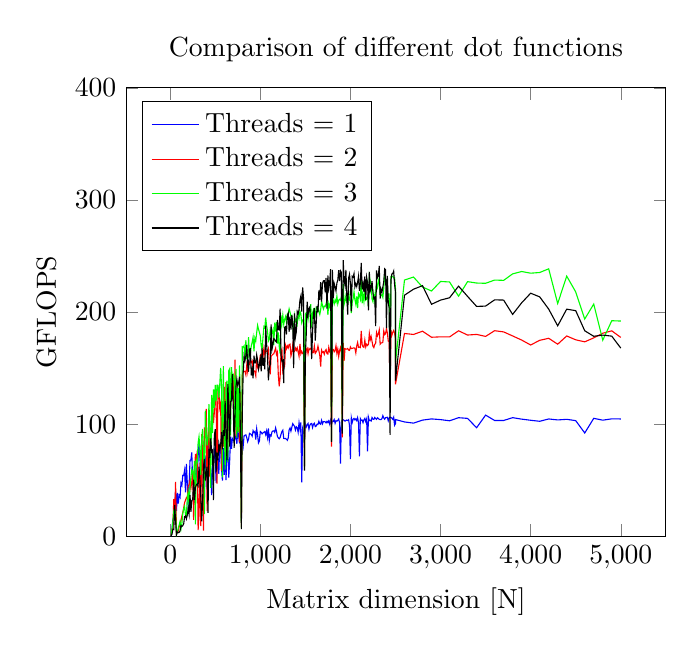
\begin{tikzpicture}
\begin{axis}[xlabel={Matrix dimension [N]}, ylabel={GFLOPS}, title={Comparison of different dot functions}, legend pos={north west}, legend entries={Threads = 1, Threads = 2, Threads = 3, Threads = 4}, ymin={0}, ymax={400}]
    \addplot[no marks, blue]
        table[row sep={\\}]
        {
            \\
            10.0  0.022595040388634694  \\
            20.0  5.988023952095808  \\
            30.0  15.066964285714285  \\
            40.0  16.45878873601646  \\
            50.0  22.841480127912288  \\
            60.0  40.24594745667971  \\
            70.0  22.63876971817042  \\
            80.0  38.70431265827569  \\
            90.0  29.17692261511677  \\
            100.0  36.48902592545292  \\
            110.0  34.78510852378899  \\
            120.0  47.51495153639926  \\
            130.0  45.50302904779164  \\
            140.0  54.38240103057028  \\
            150.0  54.16248746238716  \\
            160.0  58.83789413201178  \\
            170.0  39.166135204081634  \\
            180.0  64.58078411613911  \\
            190.0  47.95078385794432  \\
            200.0  24.475422851172603  \\
            210.0  45.093341903064655  \\
            220.0  67.56688156759226  \\
            230.0  68.09513282384646  \\
            240.0  74.81734047735021  \\
            250.0  46.54841631116089  \\
            260.0  44.87995454806606  \\
            270.0  29.620611479096798  \\
            280.0  52.03702233121214  \\
            290.0  61.240119321434676  \\
            300.0  46.439428795025826  \\
            310.0  71.2133472137727  \\
            320.0  82.44403489681287  \\
            330.0  68.55255991934769  \\
            340.0  60.06461255390747  \\
            350.0  71.09279786431432  \\
            360.0  78.39203578854514  \\
            370.0  72.16015328672525  \\
            380.0  33.45805715588831  \\
            390.0  67.33927613598631  \\
            400.0  72.2159346716601  \\
            410.0  41.57431164658004  \\
            420.0  84.81312904673376  \\
            430.0  64.87417557894085  \\
            440.0  65.20921199539009  \\
            450.0  59.08820336846528  \\
            460.0  36.64272719829164  \\
            470.0  62.33324447710512  \\
            480.0  65.23260556752786  \\
            490.0  76.753529697475  \\
            500.0  71.35145070342541  \\
            510.0  47.49215391852964  \\
            520.0  59.29685771946549  \\
            530.0  69.27358288859632  \\
            540.0  55.67075259670629  \\
            550.0  82.32599957742207  \\
            560.0  77.51716941564177  \\
            570.0  60.29216761465467  \\
            580.0  49.56830465738112  \\
            590.0  78.48069679948291  \\
            600.0  54.736396104998605  \\
            610.0  77.04305064426279  \\
            620.0  50.040654567405475  \\
            630.0  78.1107743086973  \\
            640.0  79.29530076490032  \\
            650.0  52.3698588745529  \\
            660.0  66.53319728744431  \\
            670.0  88.83247569026791  \\
            680.0  78.0200990486437  \\
            690.0  87.0591624342983  \\
            700.0  85.41365171624788  \\
            710.0  84.95452675148644  \\
            720.0  86.98674776306524  \\
            730.0  89.67117357955485  \\
            740.0  82.317126432999  \\
            750.0  94.43682856114425  \\
            760.0  89.13308764555985  \\
            770.0  83.23923634022532  \\
            780.0  82.8619928020113  \\
            790.0  85.81350423664135  \\
            800.0  85.65647237536942  \\
            810.0  80.36263525557702  \\
            820.0  89.55512121706528  \\
            830.0  90.06990579147855  \\
            840.0  90.41608202469638  \\
            850.0  87.96201272840582  \\
            860.0  84.3113338124694  \\
            870.0  86.68178885123261  \\
            880.0  91.78448628947417  \\
            890.0  91.26688932451506  \\
            900.0  90.73198307381787  \\
            910.0  89.28248995888772  \\
            920.0  94.18036901083086  \\
            930.0  92.48597516174988  \\
            940.0  93.30935134203305  \\
            950.0  86.13250798825956  \\
            960.0  95.8429915836118  \\
            970.0  90.3355475451774  \\
            980.0  83.1778412064778  \\
            990.0  84.77117808426463  \\
            1000.0  93.43844410787916  \\
            1010.0  92.77374034759639  \\
            1020.0  91.30158103601649  \\
            1030.0  92.21219453566586  \\
            1040.0  92.68735646400054  \\
            1050.0  93.4057535039412  \\
            1060.0  90.60019962204021  \\
            1070.0  93.92175097732692  \\
            1080.0  88.24309441493851  \\
            1090.0  96.15527831280743  \\
            1100.0  85.25821693681063  \\
            1110.0  90.45108280408535  \\
            1120.0  89.57306524218005  \\
            1130.0  93.07757857166357  \\
            1140.0  93.96106125724093  \\
            1150.0  94.03201295807045  \\
            1160.0  92.66446857363971  \\
            1170.0  96.72221485793588  \\
            1180.0  93.43293822244027  \\
            1190.0  88.9801088026369  \\
            1200.0  87.76064989199041  \\
            1210.0  86.9296145848297  \\
            1220.0  88.08122680837808  \\
            1230.0  90.9104676986581  \\
            1240.0  93.40497459246187  \\
            1250.0  94.59504096047003  \\
            1260.0  87.20798228545898  \\
            1270.0  87.06247808968955  \\
            1280.0  87.23010177896163  \\
            1290.0  86.3957716524752  \\
            1300.0  85.56957859319445  \\
            1310.0  87.57656357475867  \\
            1320.0  94.94751053142511  \\
            1330.0  96.54981030657325  \\
            1340.0  93.70705461527896  \\
            1350.0  97.1017416686972  \\
            1360.0  100.393583255135  \\
            1370.0  99.14099432246077  \\
            1380.0  98.09080145118155  \\
            1390.0  94.69632071642606  \\
            1400.0  97.65098144218543  \\
            1410.0  96.78139703687219  \\
            1420.0  92.73468336550032  \\
            1430.0  101.30096356932721  \\
            1440.0  95.78133562046446  \\
            1450.0  101.52549581648687  \\
            1460.0  48.12766511536991  \\
            1470.0  95.52291704938958  \\
            1480.0  92.16094961093758  \\
            1490.0  91.48099927220599  \\
            1500.0  100.35874758289674  \\
            1510.0  97.45832266999183  \\
            1520.0  99.44702505460116  \\
            1530.0  100.58559553965061  \\
            1540.0  95.43799010101023  \\
            1550.0  99.04630552925012  \\
            1560.0  100.26284553202277  \\
            1570.0  100.5874403959075  \\
            1580.0  96.95745921149168  \\
            1590.0  100.0416686914071  \\
            1600.0  100.82890045776345  \\
            1610.0  97.76413393983934  \\
            1620.0  98.2455378182748  \\
            1630.0  99.87346047430258  \\
            1640.0  99.65001188314933  \\
            1650.0  102.50009882929639  \\
            1660.0  100.4153114001322  \\
            1670.0  99.8858482804158  \\
            1680.0  103.37293228688058  \\
            1690.0  100.23963766267055  \\
            1700.0  102.17288217326733  \\
            1710.0  102.27568000971496  \\
            1720.0  101.99577514489397  \\
            1730.0  101.13240300891007  \\
            1740.0  102.49344121814883  \\
            1750.0  101.36379615145059  \\
            1760.0  102.9251726000234  \\
            1770.0  100.02530741382762  \\
            1780.0  103.60207177984724  \\
            1790.0  99.75788010667323  \\
            1800.0  102.71335774272602  \\
            1810.0  102.3801984111315  \\
            1820.0  104.07869237547972  \\
            1830.0  100.70214859667516  \\
            1840.0  103.07682853245528  \\
            1850.0  102.63937415063603  \\
            1860.0  103.28871070220029  \\
            1870.0  104.52186069829511  \\
            1880.0  101.06229702320113  \\
            1890.0  64.86819935950417  \\
            1900.0  102.80164303074442  \\
            1910.0  103.75429539269689  \\
            1920.0  103.85897289583478  \\
            1930.0  103.35760164188481  \\
            1940.0  102.63903396009388  \\
            1950.0  103.24602480438796  \\
            1960.0  103.60904513991757  \\
            1970.0  103.18706134901007  \\
            1980.0  103.92882116245974  \\
            1990.0  98.70663863101844  \\
            2000.0  68.85364224083852  \\
            2010.0  105.72193369488687  \\
            2020.0  101.43381263400943  \\
            2030.0  104.27676780284253  \\
            2040.0  105.09954964669957  \\
            2050.0  103.77880865908901  \\
            2060.0  104.7617801855412  \\
            2070.0  103.16016359163807  \\
            2080.0  105.79052990452674  \\
            2090.0  101.08393471484261  \\
            2100.0  71.28750871537135  \\
            2110.0  104.92812627461132  \\
            2120.0  103.30842129976566  \\
            2130.0  103.62937283668751  \\
            2140.0  101.30312489220769  \\
            2150.0  103.92905174206146  \\
            2160.0  105.07614139364914  \\
            2170.0  102.27082723435346  \\
            2180.0  104.65497849605536  \\
            2190.0  75.58369608515872  \\
            2200.0  106.15979816278644  \\
            2210.0  103.10563590696857  \\
            2220.0  103.42217914301786  \\
            2230.0  102.7710787333842  \\
            2240.0  105.86501568683927  \\
            2250.0  104.43452809932776  \\
            2260.0  104.24081857315677  \\
            2270.0  105.91496088642216  \\
            2280.0  104.97112432160263  \\
            2290.0  104.28225861389916  \\
            2300.0  105.68629165929815  \\
            2310.0  105.02555181418984  \\
            2320.0  104.3093926491695  \\
            2330.0  104.06998183735541  \\
            2340.0  104.04185074811446  \\
            2350.0  104.88807928829594  \\
            2360.0  107.51281244714669  \\
            2370.0  105.51351914323236  \\
            2380.0  104.4025082566325  \\
            2390.0  105.77660164532172  \\
            2400.0  105.94207924895159  \\
            2410.0  106.05973378292845  \\
            2420.0  102.94217221394156  \\
            2430.0  105.6355514810419  \\
            2440.0  106.17549955695902  \\
            2450.0  106.04543548948133  \\
            2460.0  105.34997302513915  \\
            2470.0  104.28425511567895  \\
            2480.0  106.14199873734586  \\
            2490.0  98.95372449677622  \\
            2500.0  100.36825933354474  \\
            2500.0  104.09715960523611  \\
            2600.0  101.94099133304664  \\
            2700.0  100.88355527548919  \\
            2800.0  103.5658873913934  \\
            2900.0  104.63533571926123  \\
            3000.0  104.01519894742474  \\
            3100.0  102.97575013030152  \\
            3200.0  105.71998685778738  \\
            3300.0  105.12374791303604  \\
            3400.0  96.75829171896754  \\
            3500.0  108.03273638088396  \\
            3600.0  103.26115337177417  \\
            3700.0  103.23227554965321  \\
            3800.0  105.76684488941581  \\
            3900.0  104.44662254773647  \\
            4000.0  103.43483064373966  \\
            4100.0  102.51905979349453  \\
            4200.0  104.59577136398649  \\
            4300.0  103.73782281208919  \\
            4400.0  104.27589211828759  \\
            4500.0  103.10933973332618  \\
            4600.0  92.08604814526636  \\
            4700.0  105.16559328655947  \\
            4800.0  103.5200116174704  \\
            4900.0  104.70608638037817  \\
            5000.0  104.59874529930677  \\
        }
        ;
    \addplot[no marks, red]
        table[row sep={\\}]
        {
            \\
            10.0  0.4777830864787387  \\
            20.0  5.706134094151213  \\
            30.0  7.604562737642585  \\
            40.0  33.169214822492876  \\
            50.0  16.37626097209485  \\
            60.0  48.52842057964502  \\
            70.0  2.5855375732129264  \\
            80.0  3.5524471642868045  \\
            90.0  4.687876790508496  \\
            100.0  8.461740241498067  \\
            110.0  10.7452227756743  \\
            120.0  13.897937024972855  \\
            130.0  18.02119561651027  \\
            140.0  21.04383237023034  \\
            150.0  25.267933681968426  \\
            160.0  29.93572151593441  \\
            170.0  32.12748983141732  \\
            180.0  34.37939358569648  \\
            190.0  33.537718320327016  \\
            200.0  44.87486923182638  \\
            210.0  45.97501433461331  \\
            220.0  49.65896769228976  \\
            230.0  42.65119580744389  \\
            240.0  48.718599340268966  \\
            250.0  58.47592101914642  \\
            260.0  14.678016463496618  \\
            270.0  49.37141309146366  \\
            280.0  73.42555009791968  \\
            290.0  62.675712486829596  \\
            300.0  76.41527456432681  \\
            310.0  5.474323454952094  \\
            320.0  18.323731939369743  \\
            330.0  65.58235661786512  \\
            340.0  8.9534555397399  \\
            350.0  90.9937901380771  \\
            360.0  72.99352295128134  \\
            370.0  4.9589343298781445  \\
            380.0  97.06798845557492  \\
            390.0  87.51664386012149  \\
            400.0  113.56981882064842  \\
            410.0  22.43872740532375  \\
            420.0  87.65414425168977  \\
            430.0  102.69110973484132  \\
            440.0  52.80148367805376  \\
            450.0  92.49480176676491  \\
            460.0  104.99224444976583  \\
            470.0  113.36603987023665  \\
            480.0  100.93913960956728  \\
            490.0  110.12493412572789  \\
            500.0  126.16106023736445  \\
            510.0  119.35169977043077  \\
            520.0  47.0085412936175  \\
            530.0  132.65093825610575  \\
            540.0  130.54075294882296  \\
            550.0  114.67332662237341  \\
            560.0  118.79615530573356  \\
            570.0  57.95898120408701  \\
            580.0  114.4717813025278  \\
            590.0  80.02588833337815  \\
            600.0  133.2723324478333  \\
            610.0  80.31550003060737  \\
            620.0  137.39196354323548  \\
            630.0  124.04995594573784  \\
            640.0  78.11139807406227  \\
            650.0  131.6397798757589  \\
            660.0  92.64080228373228  \\
            670.0  109.98101789568874  \\
            680.0  138.0479096914346  \\
            690.0  131.5913809005451  \\
            700.0  139.80076963788136  \\
            710.0  91.83003370718049  \\
            720.0  157.52097582921047  \\
            730.0  89.06249338213317  \\
            740.0  135.68595450604215  \\
            750.0  93.884317163088  \\
            760.0  128.29339702956784  \\
            770.0  83.67544156682624  \\
            780.0  128.77988258027068  \\
            790.0  8.310490352540956  \\
            800.0  143.61263185294516  \\
            810.0  146.824346538401  \\
            820.0  147.1468886861521  \\
            830.0  147.041185325995  \\
            840.0  143.96526785447534  \\
            850.0  152.82639556037608  \\
            860.0  146.86577696008143  \\
            870.0  155.33553915870795  \\
            880.0  153.59602450560166  \\
            890.0  156.4589540181314  \\
            900.0  155.05282377459616  \\
            910.0  156.44262843695012  \\
            920.0  148.63559790578435  \\
            930.0  147.70203542779737  \\
            940.0  146.60678019114673  \\
            950.0  143.00796349404294  \\
            960.0  159.81593825904176  \\
            970.0  150.5400021541696  \\
            980.0  148.98365123219645  \\
            990.0  154.40187828495186  \\
            1000.0  161.09633141768316  \\
            1010.0  162.35959013501378  \\
            1020.0  160.46971969650403  \\
            1030.0  159.82668878861836  \\
            1040.0  167.57636875608515  \\
            1050.0  162.05741840800084  \\
            1060.0  165.73703493887365  \\
            1070.0  164.7633358629782  \\
            1080.0  165.0614591584881  \\
            1090.0  167.36348195093115  \\
            1100.0  154.57199815024583  \\
            1110.0  144.39706222621626  \\
            1120.0  160.42205609156332  \\
            1130.0  161.5108148611974  \\
            1140.0  162.32587943856745  \\
            1150.0  162.73615668638956  \\
            1160.0  165.20290247288497  \\
            1170.0  167.64493643339966  \\
            1180.0  162.06027765425128  \\
            1190.0  164.24760568348358  \\
            1200.0  143.76188240211465  \\
            1210.0  133.6607727175125  \\
            1220.0  141.81645298373485  \\
            1230.0  164.63129155888046  \\
            1240.0  166.85349133429042  \\
            1250.0  147.19090052193658  \\
            1260.0  150.42322266445856  \\
            1270.0  151.48168606786953  \\
            1280.0  170.28307245048  \\
            1290.0  167.18589808889814  \\
            1300.0  169.78906201396723  \\
            1310.0  167.95076313274365  \\
            1320.0  171.03197781044864  \\
            1330.0  171.3443249748998  \\
            1340.0  160.7358685726427  \\
            1350.0  163.53495116533796  \\
            1360.0  170.52314099832725  \\
            1370.0  164.2408222998581  \\
            1380.0  164.85459648975342  \\
            1390.0  167.85552551623755  \\
            1400.0  165.8510710570298  \\
            1410.0  168.1165702641426  \\
            1420.0  164.4090024828258  \\
            1430.0  160.52654469031674  \\
            1440.0  171.56476841720453  \\
            1450.0  162.71628175582805  \\
            1460.0  164.84026566619212  \\
            1470.0  163.08618121980598  \\
            1480.0  163.8878098269836  \\
            1490.0  62.40975632727336  \\
            1500.0  158.5944071388629  \\
            1510.0  166.5221004041471  \\
            1520.0  167.7186829485582  \\
            1530.0  162.76023240652657  \\
            1540.0  167.49137518456197  \\
            1550.0  166.5239196342182  \\
            1560.0  167.6581970575236  \\
            1570.0  166.33850796508395  \\
            1580.0  163.66831687215083  \\
            1590.0  163.7663382699247  \\
            1600.0  169.71592512560986  \\
            1610.0  163.2160126615497  \\
            1620.0  164.45631078514134  \\
            1630.0  165.77153992269106  \\
            1640.0  169.69692959303885  \\
            1650.0  165.48903300950158  \\
            1660.0  161.37405881954294  \\
            1670.0  151.2305114843236  \\
            1680.0  165.97347004653426  \\
            1690.0  163.89042159075376  \\
            1700.0  164.53082184217155  \\
            1710.0  162.3498736955048  \\
            1720.0  165.3763216712666  \\
            1730.0  166.5500516693647  \\
            1740.0  162.94815041623272  \\
            1750.0  162.4895982023159  \\
            1760.0  168.53307768341645  \\
            1770.0  164.87212362635998  \\
            1780.0  166.51112888718538  \\
            1790.0  79.94349283935422  \\
            1800.0  166.56728418612144  \\
            1810.0  166.64970353395006  \\
            1820.0  164.51807241409762  \\
            1830.0  165.37158373451464  \\
            1840.0  169.9581561351199  \\
            1850.0  163.22884856650055  \\
            1860.0  167.01311741553525  \\
            1870.0  160.35879724924658  \\
            1880.0  165.51502048850787  \\
            1890.0  168.29549617093147  \\
            1900.0  163.4812472363083  \\
            1910.0  88.23897552754093  \\
            1920.0  172.46481152298574  \\
            1930.0  156.43248078742468  \\
            1940.0  167.2683635414282  \\
            1950.0  166.86012490889206  \\
            1960.0  166.9496634149461  \\
            1970.0  167.4770965159892  \\
            1980.0  166.074710397779  \\
            1990.0  165.77457240589692  \\
            2000.0  168.84858792031451  \\
            2010.0  167.4143921727112  \\
            2020.0  167.56002347065925  \\
            2030.0  167.8637931403981  \\
            2040.0  168.05048388825458  \\
            2050.0  167.53315443230045  \\
            2060.0  163.5269972770648  \\
            2070.0  169.7559947157466  \\
            2080.0  172.87277314508646  \\
            2090.0  168.47418801421966  \\
            2100.0  168.76818686328554  \\
            2110.0  168.35659076761627  \\
            2120.0  183.14844536632538  \\
            2130.0  171.0537284484046  \\
            2140.0  168.96676527456586  \\
            2150.0  168.53053506553056  \\
            2160.0  174.96790393204915  \\
            2170.0  168.90029556315756  \\
            2180.0  171.22987649825885  \\
            2190.0  170.13492496511904  \\
            2200.0  171.23974042094534  \\
            2210.0  180.86337013991084  \\
            2220.0  175.20149705107198  \\
            2230.0  178.05256530499383  \\
            2240.0  173.83493075818436  \\
            2250.0  169.45609971814852  \\
            2260.0  168.28389426028224  \\
            2270.0  171.17451186433848  \\
            2280.0  172.08163631534822  \\
            2290.0  181.65345058071676  \\
            2300.0  178.66714442420658  \\
            2310.0  180.4880745841039  \\
            2320.0  184.0729944043344  \\
            2330.0  171.3602114736484  \\
            2340.0  172.35783484518393  \\
            2350.0  172.53066415446764  \\
            2360.0  173.03460626040544  \\
            2370.0  183.15580222083642  \\
            2380.0  179.80966048957163  \\
            2390.0  180.7293188804798  \\
            2400.0  185.30111132344274  \\
            2410.0  181.34251859396076  \\
            2420.0  174.14390779370552  \\
            2430.0  173.74240496391408  \\
            2440.0  128.70501379134112  \\
            2450.0  183.69377486249627  \\
            2460.0  179.24707308692058  \\
            2470.0  181.99317634116957  \\
            2480.0  183.5089327739041  \\
            2490.0  181.16176504264826  \\
            2500.0  176.3073967813423  \\
            2500.0  135.47235673338753  \\
            2600.0  180.86380009651867  \\
            2700.0  179.9979061971954  \\
            2800.0  182.88864677860107  \\
            2900.0  177.5035808758287  \\
            3000.0  177.87370836265532  \\
            3100.0  177.8003680314234  \\
            3200.0  183.26771110824117  \\
            3300.0  179.471904482892  \\
            3400.0  180.038683672981  \\
            3500.0  178.25005137551045  \\
            3600.0  183.35213037188464  \\
            3700.0  182.2821121264007  \\
            3800.0  178.67371890801897  \\
            3900.0  175.01017964519528  \\
            4000.0  170.59929404839252  \\
            4100.0  174.753039814751  \\
            4200.0  176.56720514949455  \\
            4300.0  171.30834141342848  \\
            4400.0  178.6470021107721  \\
            4500.0  175.21932005199218  \\
            4600.0  173.40699464217084  \\
            4700.0  176.93911628166282  \\
            4800.0  181.08433529869077  \\
            4900.0  183.22964055570156  \\
            5000.0  177.35701655923512  \\
        }
        ;
    \addplot[no marks, green]
        table[row sep={\\}]
        {
            \\
            10.0  0.4837929366231253  \\
            20.0  6.3016935801496645  \\
            30.0  12.72984441301273  \\
            40.0  22.06516117910705  \\
            50.0  19.79727589483687  \\
            60.0  22.041940915352825  \\
            70.0  1.508630642795409  \\
            80.0  4.0400852205476205  \\
            90.0  7.257739348595493  \\
            100.0  10.164564295951454  \\
            110.0  13.247406006618727  \\
            120.0  6.3606932713951005  \\
            130.0  11.182767238614904  \\
            140.0  20.14284980216844  \\
            150.0  24.538851363633057  \\
            160.0  26.632855424428623  \\
            170.0  19.311120107856123  \\
            180.0  18.10555988463604  \\
            190.0  34.46326690064239  \\
            200.0  39.30122423313487  \\
            210.0  26.18113352632531  \\
            220.0  43.33502229222245  \\
            230.0  52.20611266771648  \\
            240.0  59.59609676605817  \\
            250.0  56.917632445054  \\
            260.0  51.78031664476747  \\
            270.0  67.28207161645494  \\
            280.0  10.62784507998601  \\
            290.0  67.75898593505818  \\
            300.0  65.98982290286787  \\
            310.0  83.41324851357766  \\
            320.0  88.75430323484083  \\
            330.0  78.07520090726003  \\
            340.0  54.62652049189441  \\
            350.0  87.83367835153342  \\
            360.0  95.77681636926297  \\
            370.0  78.38534211279703  \\
            380.0  19.607695999239592  \\
            390.0  111.91884049220971  \\
            400.0  91.54804162288929  \\
            410.0  80.8864044860085  \\
            420.0  87.52118981943616  \\
            430.0  117.80071355759429  \\
            440.0  100.08612313140416  \\
            450.0  43.0851878679676  \\
            460.0  126.08069677538022  \\
            470.0  92.04105469156897  \\
            480.0  131.0668738289347  \\
            490.0  114.42279216355256  \\
            500.0  134.90361136967636  \\
            510.0  120.41792375283512  \\
            520.0  134.694184483174  \\
            530.0  134.62237518152864  \\
            540.0  123.47420583033431  \\
            550.0  134.9100066127189  \\
            560.0  150.11049981131052  \\
            570.0  134.0107936314969  \\
            580.0  52.55443702804756  \\
            590.0  151.8288224818345  \\
            600.0  105.30213302633211  \\
            610.0  59.3429660868391  \\
            620.0  131.60145622570727  \\
            630.0  138.72814090132485  \\
            640.0  66.01478044703971  \\
            650.0  147.83140679246623  \\
            660.0  149.3452354051312  \\
            670.0  89.88534025248694  \\
            680.0  150.86608423122865  \\
            690.0  138.04212879923236  \\
            700.0  144.3255850551067  \\
            710.0  142.6705316875105  \\
            720.0  94.90665724502742  \\
            730.0  149.33849584317764  \\
            740.0  87.75181134391346  \\
            750.0  132.2081654583428  \\
            760.0  92.91097097272946  \\
            770.0  152.37580600641033  \\
            780.0  99.53298034633052  \\
            790.0  7.142719980781953  \\
            800.0  169.07996392520457  \\
            810.0  168.72321241483533  \\
            820.0  169.85039113449025  \\
            830.0  158.02045994174557  \\
            840.0  174.88975410259323  \\
            850.0  158.3255658310162  \\
            860.0  158.3111381245117  \\
            870.0  177.6277696891798  \\
            880.0  160.8655892124273  \\
            890.0  163.0049633147557  \\
            900.0  169.67812362529298  \\
            910.0  173.26084117512895  \\
            920.0  177.57300684511506  \\
            930.0  164.96194485025734  \\
            940.0  176.84132443630742  \\
            950.0  174.272704285518  \\
            960.0  181.64913332128137  \\
            970.0  188.17873900844995  \\
            980.0  184.81253012899873  \\
            990.0  181.90054868295843  \\
            1000.0  178.86375902758928  \\
            1010.0  169.89751411963556  \\
            1020.0  166.6888796406823  \\
            1030.0  177.46975824870083  \\
            1040.0  186.88040616929425  \\
            1050.0  185.79034663772234  \\
            1060.0  195.04085404147548  \\
            1070.0  187.733192837211  \\
            1080.0  183.21271496055664  \\
            1090.0  174.0550133239825  \\
            1100.0  175.62808648053652  \\
            1110.0  183.54268951718672  \\
            1120.0  180.1992669939022  \\
            1130.0  181.07311992244547  \\
            1140.0  183.92142474475997  \\
            1150.0  170.59050533655108  \\
            1160.0  190.57485344385051  \\
            1170.0  182.65784162133522  \\
            1180.0  191.2575023164639  \\
            1190.0  171.7622494552669  \\
            1200.0  181.7407450392428  \\
            1210.0  169.28998174664838  \\
            1220.0  162.9422584709362  \\
            1230.0  196.95838948706825  \\
            1240.0  189.9617545625592  \\
            1250.0  197.17448769840675  \\
            1260.0  188.97568170082423  \\
            1270.0  193.28739684282365  \\
            1280.0  195.90392435686024  \\
            1290.0  191.20048413596547  \\
            1300.0  198.28672865661554  \\
            1310.0  198.53420920348967  \\
            1320.0  202.80717249007643  \\
            1330.0  199.81275174462894  \\
            1340.0  196.458398466221  \\
            1350.0  197.0117788280891  \\
            1360.0  188.99463949834663  \\
            1370.0  178.21544883941772  \\
            1380.0  196.47582269753914  \\
            1390.0  191.82609890038265  \\
            1400.0  193.45087706602135  \\
            1410.0  189.70349238725018  \\
            1420.0  198.32756650439566  \\
            1430.0  194.62067013389506  \\
            1440.0  200.81125221550943  \\
            1450.0  198.44877808311807  \\
            1460.0  190.42973315302856  \\
            1470.0  193.01102801067074  \\
            1480.0  193.0341463408825  \\
            1490.0  62.29293412011075  \\
            1500.0  197.79018838768238  \\
            1510.0  199.37264186234188  \\
            1520.0  198.6637997626426  \\
            1530.0  193.26211504554902  \\
            1540.0  199.53256919303786  \\
            1550.0  200.13649939408845  \\
            1560.0  207.10564560987825  \\
            1570.0  186.17038587573302  \\
            1580.0  199.0558665094835  \\
            1590.0  202.35583657071894  \\
            1600.0  200.74494705094722  \\
            1610.0  197.4030078824861  \\
            1620.0  203.92426557350103  \\
            1630.0  202.97560117459014  \\
            1640.0  204.2192340524039  \\
            1650.0  200.43632059397106  \\
            1660.0  197.80619278832057  \\
            1670.0  202.13646157562576  \\
            1680.0  209.81653412249116  \\
            1690.0  205.71549439924118  \\
            1700.0  202.76104163460477  \\
            1710.0  205.32192503355847  \\
            1720.0  204.92358458969366  \\
            1730.0  207.27419258826558  \\
            1740.0  210.54332880435433  \\
            1750.0  197.47618844785808  \\
            1760.0  207.62713752484953  \\
            1770.0  204.5741711151379  \\
            1780.0  208.58929718607874  \\
            1790.0  85.24451080093357  \\
            1800.0  216.89890538017696  \\
            1810.0  210.00500085183236  \\
            1820.0  207.05497390942702  \\
            1830.0  210.75484767698472  \\
            1840.0  208.70096705088065  \\
            1850.0  214.0165552894424  \\
            1860.0  207.22545808357503  \\
            1870.0  210.61116212237027  \\
            1880.0  211.42498709472312  \\
            1890.0  210.45099259724256  \\
            1900.0  213.57465764650286  \\
            1910.0  95.21635998758202  \\
            1920.0  224.8669981839431  \\
            1930.0  206.78487760727663  \\
            1940.0  209.9393506734232  \\
            1950.0  214.66199740725042  \\
            1960.0  208.12907739069772  \\
            1970.0  208.07399572215837  \\
            1980.0  219.41985290397204  \\
            1990.0  210.7015131924414  \\
            2000.0  209.87844863412548  \\
            2010.0  199.0003423434771  \\
            2020.0  208.60249598424642  \\
            2030.0  211.9205923786402  \\
            2040.0  217.97297598112323  \\
            2050.0  210.96712932486747  \\
            2060.0  206.99392790824186  \\
            2070.0  213.87862952393084  \\
            2080.0  203.42730320631938  \\
            2090.0  216.5388854979891  \\
            2100.0  214.84289251005967  \\
            2110.0  211.6781441048871  \\
            2120.0  230.69084491178566  \\
            2130.0  207.71978137956967  \\
            2140.0  215.54955542375237  \\
            2150.0  209.35659318516286  \\
            2160.0  219.19503686401657  \\
            2170.0  210.66309796964765  \\
            2180.0  211.74508130869918  \\
            2190.0  214.2373912537282  \\
            2200.0  204.5761109205218  \\
            2210.0  232.05713701248817  \\
            2220.0  227.80013989003427  \\
            2230.0  224.1788741529829  \\
            2240.0  211.7060994664121  \\
            2250.0  209.30232750435673  \\
            2260.0  216.63345742477097  \\
            2270.0  209.88170118094448  \\
            2280.0  216.34310047546245  \\
            2290.0  224.94670622902612  \\
            2300.0  222.08256146927062  \\
            2310.0  228.64126632303984  \\
            2320.0  225.49041994168044  \\
            2330.0  216.02239051960044  \\
            2340.0  214.62222114758623  \\
            2350.0  215.4623035788504  \\
            2360.0  212.95608049459932  \\
            2370.0  221.10064766353585  \\
            2380.0  233.4423880883996  \\
            2390.0  229.57872163933632  \\
            2400.0  224.93399885853805  \\
            2410.0  222.70189569105926  \\
            2420.0  213.11105426808234  \\
            2430.0  214.90269460730326  \\
            2440.0  144.66327913679223  \\
            2450.0  231.78234394956058  \\
            2460.0  232.0128324983815  \\
            2470.0  231.70781230022916  \\
            2480.0  230.3263875210961  \\
            2490.0  230.51456035891243  \\
            2500.0  220.99435636281223  \\
            2500.0  155.1335919647769  \\
            2600.0  228.51383428876477  \\
            2700.0  231.21858118708099  \\
            2800.0  222.31652175026176  \\
            2900.0  218.78021905139565  \\
            3000.0  227.26918336563816  \\
            3100.0  226.8203735905374  \\
            3200.0  214.13452826603873  \\
            3300.0  227.11439563525528  \\
            3400.0  225.87813703247977  \\
            3500.0  225.6323834332784  \\
            3600.0  228.5285839402581  \\
            3700.0  228.25895731535417  \\
            3800.0  234.0414031235937  \\
            3900.0  236.15925906976275  \\
            4000.0  234.66486381473956  \\
            4100.0  235.2638147483957  \\
            4200.0  238.54745733156147  \\
            4300.0  207.59074879831923  \\
            4400.0  232.04453149867496  \\
            4500.0  217.95156035719643  \\
            4600.0  193.77174750607637  \\
            4700.0  207.1369462478727  \\
            4800.0  174.87051498683576  \\
            4900.0  192.2461736691283  \\
            5000.0  191.97078682554985  \\
        }
        ;
    \addplot[no marks, black]
        table[row sep={\\}]
        {
            \\
            10.0  0.4081632653061224  \\
            20.0  1.7615325333039744  \\
            30.0  6.0934326337169935  \\
            40.0  5.909237800655555  \\
            50.0  28.017482909335424  \\
            60.0  13.543168850711643  \\
            70.0  1.139470528242591  \\
            80.0  3.7223098677562176  \\
            90.0  3.1449864644786936  \\
            100.0  3.413277992719478  \\
            110.0  4.964121078307052  \\
            120.0  9.543850347124419  \\
            130.0  8.640744433366567  \\
            140.0  9.369392747939775  \\
            150.0  11.054338213618944  \\
            160.0  17.43345938825412  \\
            170.0  18.12279828104539  \\
            180.0  15.45432864297639  \\
            190.0  18.85793860378671  \\
            200.0  24.755232637298707  \\
            210.0  19.58824705176894  \\
            220.0  36.950603553129504  \\
            230.0  21.676349493945338  \\
            240.0  31.813683750258903  \\
            250.0  32.56551660893452  \\
            260.0  50.395326332389516  \\
            270.0  32.48748894141259  \\
            280.0  43.22148945993811  \\
            290.0  45.67425188725357  \\
            300.0  46.65299330788729  \\
            310.0  44.93776953837382  \\
            320.0  62.115192138546  \\
            330.0  50.45520884008618  \\
            340.0  34.83141935109378  \\
            350.0  13.248573364264697  \\
            360.0  30.849522290624634  \\
            370.0  62.794077995171406  \\
            380.0  69.00103051364094  \\
            390.0  49.71502635183864  \\
            400.0  56.4448560215196  \\
            410.0  61.94839805672529  \\
            420.0  20.763651614691444  \\
            430.0  77.83776904287554  \\
            440.0  69.79526155197446  \\
            450.0  87.23647762797196  \\
            460.0  75.2237813984671  \\
            470.0  76.5632627897956  \\
            480.0  32.241738404379134  \\
            490.0  89.24777106253921  \\
            500.0  95.42367155935638  \\
            510.0  57.21475167626313  \\
            520.0  74.57298654447858  \\
            530.0  67.66673461656373  \\
            540.0  82.44046045277753  \\
            550.0  77.10760397998052  \\
            560.0  81.52413969346281  \\
            570.0  92.92431374782389  \\
            580.0  77.4185458985177  \\
            590.0  94.63861654976559  \\
            600.0  89.4232387399686  \\
            610.0  120.40886209140116  \\
            620.0  92.29255976238329  \\
            630.0  67.69311652506123  \\
            640.0  135.57614456890428  \\
            650.0  116.37212213383991  \\
            660.0  79.91668534889956  \\
            670.0  120.21131496301388  \\
            680.0  120.59935307179668  \\
            690.0  144.57502049740367  \\
            700.0  115.66447724714499  \\
            710.0  78.84927220877694  \\
            720.0  109.5088038068486  \\
            730.0  133.67094366359552  \\
            740.0  140.0131643277814  \\
            750.0  134.18095942367788  \\
            760.0  137.06313226363085  \\
            770.0  142.30120415832351  \\
            780.0  87.68181474262202  \\
            790.0  6.3711706373311205  \\
            800.0  109.17575291821244  \\
            810.0  145.6344481931171  \\
            820.0  160.60805064719568  \\
            830.0  156.64624758231102  \\
            840.0  161.11489559270692  \\
            850.0  170.55806125509625  \\
            860.0  153.27937779835247  \\
            870.0  146.76205599665693  \\
            880.0  166.96598458116645  \\
            890.0  167.37747845306018  \\
            900.0  143.44932460752148  \\
            910.0  148.36133754782898  \\
            920.0  140.92980901427157  \\
            930.0  161.09511278312192  \\
            940.0  154.69745179184577  \\
            950.0  154.60003512592138  \\
            960.0  161.86568823049967  \\
            970.0  156.89485799581044  \\
            980.0  148.98733027061408  \\
            990.0  152.74018824700582  \\
            1000.0  158.25700795660848  \\
            1010.0  147.11475868162572  \\
            1020.0  167.75782730906744  \\
            1030.0  151.9798090347935  \\
            1040.0  159.01934976406804  \\
            1050.0  148.89304029459504  \\
            1060.0  187.77605349858666  \\
            1070.0  171.6052455851022  \\
            1080.0  160.14696207399592  \\
            1090.0  139.11783435658742  \\
            1100.0  149.70404208224488  \\
            1110.0  153.27495919269995  \\
            1120.0  188.9534060731392  \\
            1130.0  166.7637020231915  \\
            1140.0  171.0237368471328  \\
            1150.0  176.26987617790928  \\
            1160.0  175.56715145812834  \\
            1170.0  174.08043187595956  \\
            1180.0  173.19559895679882  \\
            1190.0  192.99946469176027  \\
            1200.0  184.39513487095542  \\
            1210.0  184.08685025567345  \\
            1220.0  203.12799673133432  \\
            1230.0  161.44223594304577  \\
            1240.0  156.01696787957437  \\
            1250.0  156.8131914407958  \\
            1260.0  136.53945526697336  \\
            1270.0  186.41158899270656  \\
            1280.0  186.9847120093573  \\
            1290.0  180.00101878398698  \\
            1300.0  196.5984178435838  \\
            1310.0  199.0282097344847  \\
            1320.0  182.40934773673445  \\
            1330.0  195.86147368580546  \\
            1340.0  184.29329830226945  \\
            1350.0  197.2516925584191  \\
            1360.0  189.85902598087526  \\
            1370.0  149.99266181000598  \\
            1380.0  198.73831097405835  \\
            1390.0  177.53378586632567  \\
            1400.0  182.38698703410645  \\
            1410.0  200.49222216949454  \\
            1420.0  198.43965743736698  \\
            1430.0  201.94736266540048  \\
            1440.0  210.6183239770144  \\
            1450.0  214.24475600624092  \\
            1460.0  200.34810894005997  \\
            1470.0  222.00685263412038  \\
            1480.0  212.25041053316707  \\
            1490.0  58.44526364286622  \\
            1500.0  161.05296476080008  \\
            1510.0  180.27833265773813  \\
            1520.0  209.32519006672635  \\
            1530.0  197.88787482550163  \\
            1540.0  203.13207914459323  \\
            1550.0  204.53509737411292  \\
            1560.0  186.56002918587757  \\
            1570.0  158.03858968017045  \\
            1580.0  182.2025978815727  \\
            1590.0  198.83727297536697  \\
            1600.0  203.6281657226037  \\
            1610.0  174.50805881909696  \\
            1620.0  189.13352216013928  \\
            1630.0  205.4995041222235  \\
            1640.0  199.85583555412038  \\
            1650.0  219.32078360569054  \\
            1660.0  210.9890409955529  \\
            1670.0  226.73073660034436  \\
            1680.0  209.37355401481986  \\
            1690.0  225.42033601195004  \\
            1700.0  227.86911648770808  \\
            1710.0  228.0038519169265  \\
            1720.0  217.62379883084122  \\
            1730.0  230.5503682350663  \\
            1740.0  203.03916017095912  \\
            1750.0  232.66964680622803  \\
            1760.0  220.82568585303656  \\
            1770.0  226.5972241760048  \\
            1780.0  238.2963109580793  \\
            1790.0  84.10497161148395  \\
            1800.0  237.53621184971715  \\
            1810.0  212.47745777282938  \\
            1820.0  225.48236542826749  \\
            1830.0  222.38831880606125  \\
            1840.0  218.75015033686168  \\
            1850.0  225.90938820064468  \\
            1860.0  228.50345177546006  \\
            1870.0  237.40473382469517  \\
            1880.0  227.50963128849088  \\
            1890.0  236.79617543992933  \\
            1900.0  235.4617071430342  \\
            1910.0  91.42805144720734  \\
            1920.0  246.38235069643363  \\
            1930.0  229.05672201114092  \\
            1940.0  223.71077094318744  \\
            1950.0  237.53325421511306  \\
            1960.0  214.18762729374808  \\
            1970.0  197.72197126506742  \\
            1980.0  230.3206888952788  \\
            1990.0  233.73358303950417  \\
            2000.0  225.66167918155782  \\
            2010.0  200.51785830627026  \\
            2020.0  231.79566095052328  \\
            2030.0  231.03391569089968  \\
            2040.0  234.291156615928  \\
            2050.0  222.49177957745434  \\
            2060.0  225.3815056092803  \\
            2070.0  222.7253511318561  \\
            2080.0  226.59709043116504  \\
            2090.0  231.98378514903192  \\
            2100.0  219.00303344386316  \\
            2110.0  225.49297996718755  \\
            2120.0  243.77309215642728  \\
            2130.0  220.14280150117497  \\
            2140.0  225.4700165887193  \\
            2150.0  217.98240245641853  \\
            2160.0  231.73055136990445  \\
            2170.0  210.88973103002763  \\
            2180.0  231.0013915738421  \\
            2190.0  226.55034369580255  \\
            2200.0  201.57055225362097  \\
            2210.0  235.80303381527648  \\
            2220.0  218.5643239564536  \\
            2230.0  221.1191334120447  \\
            2240.0  227.55566151968364  \\
            2250.0  216.9930837964067  \\
            2260.0  211.96176009605358  \\
            2270.0  212.91729888081508  \\
            2280.0  187.42730331146632  \\
            2290.0  237.1163646120492  \\
            2300.0  230.67023438651444  \\
            2310.0  232.55190843058165  \\
            2320.0  241.1332860934471  \\
            2330.0  212.0764202192454  \\
            2340.0  220.35271746955863  \\
            2350.0  217.7371428506236  \\
            2360.0  222.39863781795384  \\
            2370.0  226.86803339967474  \\
            2380.0  238.50363070709176  \\
            2390.0  237.73910994038008  \\
            2400.0  185.66668752014445  \\
            2410.0  232.17494561168033  \\
            2420.0  208.64642254114068  \\
            2430.0  203.60985774100385  \\
            2440.0  90.46387168628368  \\
            2450.0  228.73501064279125  \\
            2460.0  234.01424850615442  \\
            2470.0  234.28834518475776  \\
            2480.0  236.51915875581926  \\
            2490.0  224.67994103287245  \\
            2500.0  217.80723965894438  \\
            2500.0  138.77679794401087  \\
            2600.0  215.00012021584442  \\
            2700.0  220.33674211053582  \\
            2800.0  223.5401425708928  \\
            2900.0  206.91592358866174  \\
            3000.0  210.6370632553126  \\
            3100.0  212.73195654224102  \\
            3200.0  223.10600226568883  \\
            3300.0  213.94474232432904  \\
            3400.0  205.0184461570384  \\
            3500.0  205.2980987049796  \\
            3600.0  210.88225286176066  \\
            3700.0  210.67278878943267  \\
            3800.0  197.8886515698071  \\
            3900.0  208.20996142562888  \\
            4000.0  216.80013441879336  \\
            4100.0  213.5616933689381  \\
            4200.0  202.62850313463596  \\
            4300.0  187.700788002763  \\
            4400.0  202.56729842747123  \\
            4500.0  201.22416478945865  \\
            4600.0  183.28289596834975  \\
            4700.0  178.3586645381464  \\
            4800.0  179.428977500482  \\
            4900.0  178.49245682721192  \\
            5000.0  167.81510779055702  \\
        }
        ;
\end{axis}
\end{tikzpicture}

        \end{center}
        \caption{}
        \label{}
    \end{figure}


    \paragraph*{Speed-up} The following code investigates how performance scales as more threads are added, 
    referred to as "speed-up." The goal here is to observe how performance increases with parallelism, plotted as 
    a curve representing the speed-up as more cores are utilized. The expected behavior is not a linear speed-up—where the 
    slope of the curve remains constant—but rather a diminishing rate of performance gain. This is because of the law of 
    diminishing returns in parallel computing: as the number of threads increases, factors such as communication between 
    threads, memory access contention, and overheads from parallelization begin to outweigh the benefits of adding more 
    threads. Hence, while performance improves, the slope of the curve flattens, though it should never turn negative.
    \par

    \vspace*{0.5cm}

    \lstinputlisting[language=Julia]{code/3-speed-up/speedup.jl}

    \begin{figure}[h]
        \begin{center}
            % Recommended preamble:
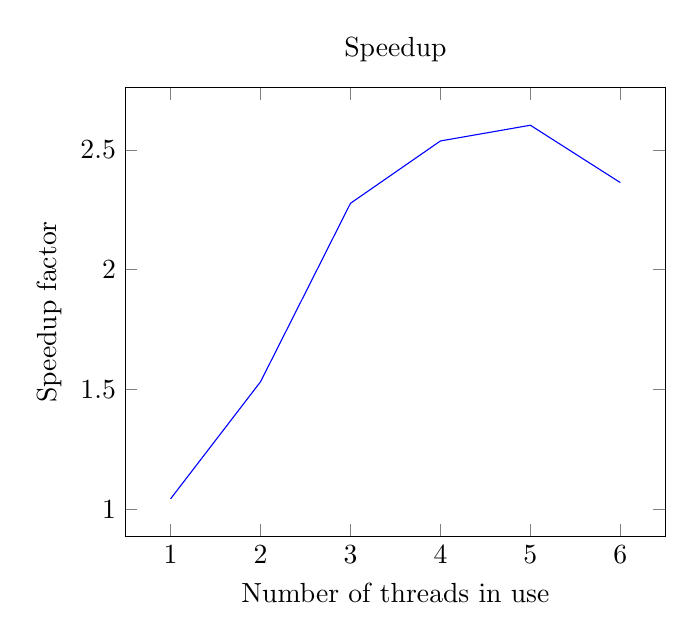
\begin{tikzpicture}
\begin{axis}[xlabel={Number of threads in use}, ylabel={Speedup factor}, title={Speedup}]
    \addplot[no marks, blue]
        table[row sep={\\}]
        {
            \\
            1.0  1.0436587518312022  \\
            2.0  1.5321710544393923  \\
            3.0  2.276699075208266  \\
            4.0  2.536789153620059  \\
            5.0  2.602390829533416  \\
            6.0  2.3630888576592275  \\
        }
        ;
\end{axis}
\end{tikzpicture}

        \end{center}
        \caption{}
        \label{}
    \end{figure}


\subsection{Theoretical time}
% \addcontentsline{toc}{subsection}{Theoretical time}

    \paragraph*{}
    In this part, we display the trend towards the theoretically expected execution time as the size of the matrices increases. 
    This code shows how, as the dimensions of the matrices grow, the observed execution times begin to approach these theoretical 
    predictions.
    \par

    \vspace*{0.5cm}

    \lstinputlisting[language=Julia]{code/4-matmul_vs_theoretical-time/matmul_vs_theoretical-time.jl}

    \begin{center}
        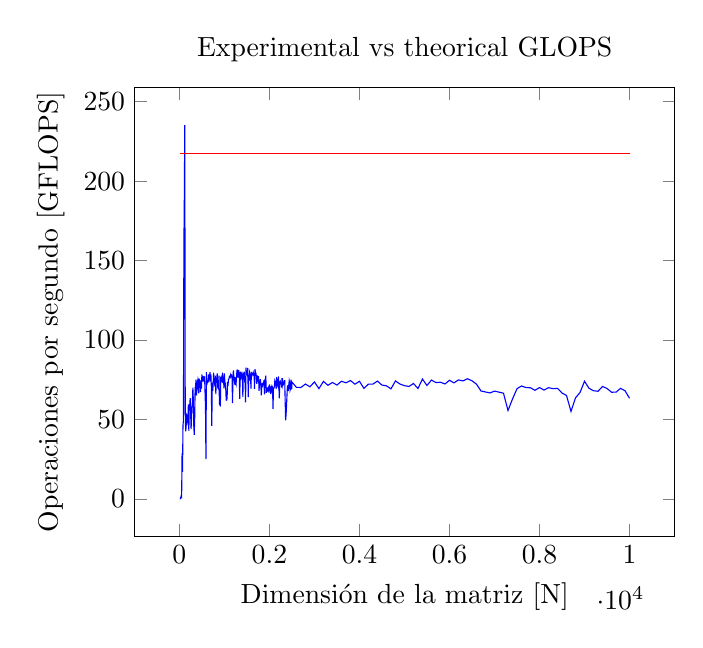
\begin{tikzpicture}
\begin{axis}[xlabel={Dimensión de la matriz [N]}, ylabel={Operaciones por segundo [GFLOPS]}, title={Experimental vs theorical GLOPS}]
    \addplot[no marks, blue]
        table[row sep={\\}]
        {
            \\
            10.0  0.0007809675094087061  \\
            20.0  0.07571348125854734  \\
            30.0  0.7329786078835921  \\
            40.0  1.8275271273557965  \\
            50.0  1.2633791855752419  \\
            60.0  28.79040319893369  \\
            70.0  17.037552155771905  \\
            80.0  46.2950404629504  \\
            90.0  49.090909090909086  \\
            100.0  158.78056525881232  \\
            110.0  190.21078956770273  \\
            120.0  235.15003061849356  \\
            130.0  55.050929000087706  \\
            140.0  42.49881904702904  \\
            150.0  45.22037395574433  \\
            160.0  52.47010446623582  \\
            170.0  51.567329845130075  \\
            180.0  49.211452294762424  \\
            190.0  51.61994355597366  \\
            200.0  59.395649268691066  \\
            210.0  42.72792494353925  \\
            220.0  58.853278577528194  \\
            230.0  59.08217944142162  \\
            240.0  63.3913258802058  \\
            250.0  54.15343878668571  \\
            260.0  43.874298238388015  \\
            270.0  50.96159821040204  \\
            280.0  58.2605695480241  \\
            290.0  61.36616394168591  \\
            300.0  70.00812872161268  \\
            310.0  61.657004840916194  \\
            320.0  45.78419475608333  \\
            330.0  40.31950885526904  \\
            340.0  50.63176994131564  \\
            350.0  70.16857642483124  \\
            360.0  70.61686837437111  \\
            370.0  75.07952177251289  \\
            380.0  65.06579267215363  \\
            390.0  68.84241934351404  \\
            400.0  73.26070221527772  \\
            410.0  74.78926487950552  \\
            420.0  70.97809477733124  \\
            430.0  66.34531657906935  \\
            440.0  75.57850150786138  \\
            450.0  72.80235747815031  \\
            460.0  72.3395416053067  \\
            470.0  67.25339488009297  \\
            480.0  74.76360047254555  \\
            490.0  69.33233542638423  \\
            500.0  78.3491029184414  \\
            510.0  73.88058392233602  \\
            520.0  76.55614932499938  \\
            530.0  76.82663679821326  \\
            540.0  73.87144368418954  \\
            550.0  76.65519353622214  \\
            560.0  76.74033606670382  \\
            570.0  67.0422914560203  \\
            580.0  57.82202196005191  \\
            590.0  24.931378589464394  \\
            600.0  79.77904160255412  \\
            610.0  71.66482806263336  \\
            620.0  73.99532794428306  \\
            630.0  73.68968270176937  \\
            640.0  75.14183112350429  \\
            650.0  78.34245200963188  \\
            660.0  75.28946912198425  \\
            670.0  76.9369199523536  \\
            680.0  79.69358602888548  \\
            690.0  73.87002200524294  \\
            700.0  78.35056303331349  \\
            710.0  70.491735152236  \\
            720.0  45.86375240739911  \\
            730.0  73.08625247547725  \\
            740.0  67.99380977525954  \\
            750.0  71.75065213370495  \\
            760.0  79.3589829924763  \\
            770.0  74.96479249348786  \\
            780.0  73.04784478980034  \\
            790.0  70.59691412793826  \\
            800.0  77.58559684008412  \\
            810.0  65.99084047268346  \\
            820.0  75.14241636275423  \\
            830.0  75.48467298241403  \\
            840.0  78.97093057959769  \\
            850.0  71.4588205492587  \\
            860.0  72.37131910888029  \\
            870.0  68.7046376045113  \\
            880.0  77.4886108950507  \\
            890.0  59.117886290844034  \\
            900.0  60.87629802630524  \\
            910.0  58.137198885784244  \\
            920.0  76.93654830372155  \\
            930.0  74.59826284522727  \\
            940.0  76.20049630359465  \\
            950.0  74.95851435830944  \\
            960.0  79.45458314040015  \\
            970.0  73.06600035633437  \\
            980.0  76.6118051639091  \\
            990.0  69.58302528129683  \\
            1000.0  78.90671588867605  \\
            1010.0  73.73565974135649  \\
            1020.0  72.52902788085167  \\
            1030.0  69.2369036060086  \\
            1040.0  62.21051675094861  \\
            1050.0  62.10134870369318  \\
            1060.0  63.437611345560505  \\
            1070.0  73.55062105915721  \\
            1080.0  70.90660523324826  \\
            1090.0  75.2282931515293  \\
            1100.0  75.29039408836343  \\
            1110.0  76.9646344940852  \\
            1120.0  77.27992410007455  \\
            1130.0  76.64235970784482  \\
            1140.0  78.12110790210953  \\
            1150.0  77.22720282423948  \\
            1160.0  77.67277652772341  \\
            1170.0  75.91295656715448  \\
            1180.0  60.262801951149015  \\
            1190.0  75.77689053484848  \\
            1200.0  80.84422896068124  \\
            1210.0  76.54710678102781  \\
            1220.0  74.4721030028837  \\
            1230.0  76.67032377151179  \\
            1240.0  71.5538059007541  \\
            1250.0  74.05595272506854  \\
            1260.0  72.45781194342484  \\
            1270.0  76.97130072826675  \\
            1280.0  81.31827336555041  \\
            1290.0  76.30869486882273  \\
            1300.0  78.79157748520453  \\
            1310.0  76.51291658818143  \\
            1320.0  81.03393552896192  \\
            1330.0  77.71355684674951  \\
            1340.0  62.87583740018239  \\
            1350.0  76.57526799126254  \\
            1360.0  79.96751268932253  \\
            1370.0  76.90300087041588  \\
            1380.0  78.15842385543871  \\
            1390.0  76.29007100102142  \\
            1400.0  77.48954872419417  \\
            1410.0  64.26176220194652  \\
            1420.0  79.2048094806947  \\
            1430.0  77.5332079606173  \\
            1440.0  80.03449703650986  \\
            1450.0  74.81340575248925  \\
            1460.0  75.51045243305968  \\
            1470.0  60.745109047772665  \\
            1480.0  82.56051718288955  \\
            1490.0  78.39297701848854  \\
            1500.0  78.61506117824061  \\
            1510.0  77.8127986812091  \\
            1520.0  82.38456196868862  \\
            1530.0  64.02909244927305  \\
            1540.0  78.00440372656401  \\
            1550.0  74.20012657085536  \\
            1560.0  79.58587595638413  \\
            1570.0  78.508152916728  \\
            1580.0  78.01729275536587  \\
            1590.0  69.38887317013338  \\
            1600.0  79.82455124901841  \\
            1610.0  77.4442843012235  \\
            1620.0  78.1152662306088  \\
            1630.0  78.4029754970414  \\
            1640.0  79.50572657584839  \\
            1650.0  78.05762311611835  \\
            1660.0  78.42128722784622  \\
            1670.0  69.15288982051649  \\
            1680.0  81.55223596065916  \\
            1690.0  79.38775099022745  \\
            1700.0  79.08815876407793  \\
            1710.0  77.24516616672872  \\
            1720.0  72.45861175129214  \\
            1730.0  77.65100111566052  \\
            1740.0  75.34319074642235  \\
            1750.0  74.25982277239896  \\
            1760.0  77.29973940325127  \\
            1770.0  67.92523302964722  \\
            1780.0  73.90104300381377  \\
            1790.0  71.50607242984884  \\
            1800.0  75.35561093879983  \\
            1810.0  71.39743667551888  \\
            1820.0  65.20335166647898  \\
            1830.0  70.88642450261982  \\
            1840.0  72.21928317732552  \\
            1850.0  71.35753850688208  \\
            1860.0  72.374795648397  \\
            1870.0  72.78461646992501  \\
            1880.0  74.61539982684555  \\
            1890.0  65.71343799646144  \\
            1900.0  73.68831627751594  \\
            1910.0  72.79760281246752  \\
            1920.0  77.60503093812218  \\
            1930.0  66.74895320268367  \\
            1940.0  70.15361839957784  \\
            1950.0  67.68738746411282  \\
            1960.0  67.9385256684973  \\
            1970.0  69.63041102137798  \\
            1980.0  70.18380977350613  \\
            1990.0  66.95046294637686  \\
            2000.0  71.97073338915024  \\
            2010.0  67.92507714184885  \\
            2020.0  70.46066422729423  \\
            2030.0  65.9216131554699  \\
            2040.0  71.01076770771876  \\
            2050.0  66.95400358945191  \\
            2060.0  70.82419347201484  \\
            2070.0  70.23023237814414  \\
            2080.0  56.71033079240754  \\
            2090.0  69.70234202347211  \\
            2100.0  69.66553696813266  \\
            2110.0  70.58637313820874  \\
            2120.0  74.35413187687762  \\
            2130.0  73.50081630836948  \\
            2140.0  72.97091473615517  \\
            2150.0  69.12422940746892  \\
            2160.0  76.60811861429066  \\
            2170.0  72.4104148752996  \\
            2180.0  71.45457634121676  \\
            2190.0  70.74325796473623  \\
            2200.0  77.01601006112043  \\
            2210.0  71.25188977706915  \\
            2220.0  63.2010859540616  \\
            2230.0  73.6129603484736  \\
            2240.0  74.0744126350192  \\
            2250.0  72.5789650059427  \\
            2260.0  72.73366309667213  \\
            2270.0  70.04597104760127  \\
            2280.0  76.02178743324438  \\
            2290.0  71.96887830086891  \\
            2300.0  73.79153727574017  \\
            2310.0  72.04156910981689  \\
            2320.0  72.66610212648257  \\
            2330.0  72.83354408665562  \\
            2340.0  74.69031834665209  \\
            2350.0  61.530698152051485  \\
            2360.0  49.38948334524575  \\
            2370.0  52.79658243117585  \\
            2380.0  58.39169078359574  \\
            2390.0  65.03253277470698  \\
            2400.0  70.92515003768104  \\
            2410.0  71.1643695861984  \\
            2420.0  67.88477482190392  \\
            2430.0  71.33411967086793  \\
            2440.0  74.33515320113385  \\
            2450.0  72.92317187901303  \\
            2460.0  68.5424098073408  \\
            2470.0  69.66841522061517  \\
            2480.0  74.9637675957147  \\
            2490.0  69.37574600305217  \\
            2500.0  69.62335589151601  \\
            2500.0  73.53280673113807  \\
            2600.0  70.17971187063652  \\
            2700.0  70.08430490637063  \\
            2800.0  72.26571450091622  \\
            2900.0  70.52248882766214  \\
            3000.0  73.57952248533184  \\
            3100.0  69.37803774533441  \\
            3200.0  73.91793711964995  \\
            3300.0  71.4666582007867  \\
            3400.0  73.2539356270529  \\
            3500.0  71.61619213123541  \\
            3600.0  74.00764830404398  \\
            3700.0  73.04693381731408  \\
            3800.0  74.45672645875693  \\
            3900.0  72.16976861158464  \\
            4000.0  73.98956561572861  \\
            4100.0  69.51664450506951  \\
            4200.0  72.23145604898944  \\
            4300.0  72.22988682673623  \\
            4400.0  74.12451712212497  \\
            4500.0  71.59103889486344  \\
            4600.0  71.14438815264845  \\
            4700.0  69.22621354809047  \\
            4800.0  74.20272260304505  \\
            4900.0  72.26349267271516  \\
            5000.0  71.24378394280423  \\
            5100.0  70.71610469558563  \\
            5200.0  72.61742906259784  \\
            5300.0  69.45596049167199  \\
            5400.0  75.41023488162787  \\
            5500.0  71.33918958780964  \\
            5600.0  74.77519782725304  \\
            5700.0  73.17985823074268  \\
            5800.0  73.38923983257662  \\
            5900.0  72.30712045999678  \\
            6000.0  74.63958444353308  \\
            6100.0  73.01080132421163  \\
            6200.0  74.84558076611452  \\
            6300.0  74.22464969136071  \\
            6400.0  75.58731085204572  \\
            6500.0  74.32142593317018  \\
            6600.0  72.20070028084432  \\
            6700.0  67.88416860501438  \\
            6800.0  67.27690019457135  \\
            6900.0  66.65464974759372  \\
            7000.0  67.82755391269934  \\
            7100.0  67.16812148688943  \\
            7200.0  66.48211188732262  \\
            7300.0  55.62463703293204  \\
            7400.0  62.8005642850087  \\
            7500.0  69.3187935877637  \\
            7600.0  71.05615152434504  \\
            7700.0  70.02400918192188  \\
            7800.0  69.9127637308178  \\
            7900.0  68.31684413268924  \\
            8000.0  70.05393273862937  \\
            8100.0  68.4540973667193  \\
            8200.0  69.96836641677375  \\
            8300.0  69.33380714047992  \\
            8400.0  69.56221223175802  \\
            8500.0  66.61520433459319  \\
            8600.0  65.05634736682968  \\
            8700.0  54.99786201358163  \\
            8800.0  63.576737342727824  \\
            8900.0  66.90018497355624  \\
            9000.0  73.98580161904891  \\
            9100.0  69.5654639719296  \\
            9200.0  68.04999353046249  \\
            9300.0  67.70077276495131  \\
            9400.0  70.73609891581741  \\
            9500.0  69.4773515246386  \\
            9600.0  67.11992556101532  \\
            9700.0  67.1345612828053  \\
            9800.0  69.54203489516685  \\
            9900.0  68.04520744843225  \\
            10000.0  63.28735592236929  \\
        }
        ;
    \addplot[no marks, red]
        table[row sep={\\}]
        {
            \\
            10.0  217.6  \\
            20.0  217.6  \\
            30.0  217.6  \\
            40.0  217.6  \\
            50.0  217.6  \\
            60.0  217.6  \\
            70.0  217.6  \\
            80.0  217.6  \\
            90.0  217.6  \\
            100.0  217.6  \\
            110.0  217.6  \\
            120.0  217.6  \\
            130.0  217.6  \\
            140.0  217.6  \\
            150.0  217.6  \\
            160.0  217.6  \\
            170.0  217.6  \\
            180.0  217.6  \\
            190.0  217.6  \\
            200.0  217.6  \\
            210.0  217.6  \\
            220.0  217.6  \\
            230.0  217.6  \\
            240.0  217.6  \\
            250.0  217.6  \\
            260.0  217.6  \\
            270.0  217.6  \\
            280.0  217.6  \\
            290.0  217.6  \\
            300.0  217.6  \\
            310.0  217.6  \\
            320.0  217.6  \\
            330.0  217.6  \\
            340.0  217.6  \\
            350.0  217.6  \\
            360.0  217.6  \\
            370.0  217.6  \\
            380.0  217.6  \\
            390.0  217.6  \\
            400.0  217.6  \\
            410.0  217.6  \\
            420.0  217.6  \\
            430.0  217.6  \\
            440.0  217.6  \\
            450.0  217.6  \\
            460.0  217.6  \\
            470.0  217.6  \\
            480.0  217.6  \\
            490.0  217.6  \\
            500.0  217.6  \\
            510.0  217.6  \\
            520.0  217.6  \\
            530.0  217.6  \\
            540.0  217.6  \\
            550.0  217.6  \\
            560.0  217.6  \\
            570.0  217.6  \\
            580.0  217.6  \\
            590.0  217.6  \\
            600.0  217.6  \\
            610.0  217.6  \\
            620.0  217.6  \\
            630.0  217.6  \\
            640.0  217.6  \\
            650.0  217.6  \\
            660.0  217.6  \\
            670.0  217.6  \\
            680.0  217.6  \\
            690.0  217.6  \\
            700.0  217.6  \\
            710.0  217.6  \\
            720.0  217.6  \\
            730.0  217.6  \\
            740.0  217.6  \\
            750.0  217.6  \\
            760.0  217.6  \\
            770.0  217.6  \\
            780.0  217.6  \\
            790.0  217.6  \\
            800.0  217.6  \\
            810.0  217.6  \\
            820.0  217.6  \\
            830.0  217.6  \\
            840.0  217.6  \\
            850.0  217.6  \\
            860.0  217.6  \\
            870.0  217.6  \\
            880.0  217.6  \\
            890.0  217.6  \\
            900.0  217.6  \\
            910.0  217.6  \\
            920.0  217.6  \\
            930.0  217.6  \\
            940.0  217.6  \\
            950.0  217.6  \\
            960.0  217.6  \\
            970.0  217.6  \\
            980.0  217.6  \\
            990.0  217.6  \\
            1000.0  217.6  \\
            1010.0  217.6  \\
            1020.0  217.6  \\
            1030.0  217.6  \\
            1040.0  217.6  \\
            1050.0  217.6  \\
            1060.0  217.6  \\
            1070.0  217.6  \\
            1080.0  217.6  \\
            1090.0  217.6  \\
            1100.0  217.6  \\
            1110.0  217.6  \\
            1120.0  217.6  \\
            1130.0  217.6  \\
            1140.0  217.6  \\
            1150.0  217.6  \\
            1160.0  217.6  \\
            1170.0  217.6  \\
            1180.0  217.6  \\
            1190.0  217.6  \\
            1200.0  217.6  \\
            1210.0  217.6  \\
            1220.0  217.6  \\
            1230.0  217.6  \\
            1240.0  217.6  \\
            1250.0  217.6  \\
            1260.0  217.6  \\
            1270.0  217.6  \\
            1280.0  217.6  \\
            1290.0  217.6  \\
            1300.0  217.6  \\
            1310.0  217.6  \\
            1320.0  217.6  \\
            1330.0  217.6  \\
            1340.0  217.6  \\
            1350.0  217.6  \\
            1360.0  217.6  \\
            1370.0  217.6  \\
            1380.0  217.6  \\
            1390.0  217.6  \\
            1400.0  217.6  \\
            1410.0  217.6  \\
            1420.0  217.6  \\
            1430.0  217.6  \\
            1440.0  217.6  \\
            1450.0  217.6  \\
            1460.0  217.6  \\
            1470.0  217.6  \\
            1480.0  217.6  \\
            1490.0  217.6  \\
            1500.0  217.6  \\
            1510.0  217.6  \\
            1520.0  217.6  \\
            1530.0  217.6  \\
            1540.0  217.6  \\
            1550.0  217.6  \\
            1560.0  217.6  \\
            1570.0  217.6  \\
            1580.0  217.6  \\
            1590.0  217.6  \\
            1600.0  217.6  \\
            1610.0  217.6  \\
            1620.0  217.6  \\
            1630.0  217.6  \\
            1640.0  217.6  \\
            1650.0  217.6  \\
            1660.0  217.6  \\
            1670.0  217.6  \\
            1680.0  217.6  \\
            1690.0  217.6  \\
            1700.0  217.6  \\
            1710.0  217.6  \\
            1720.0  217.6  \\
            1730.0  217.6  \\
            1740.0  217.6  \\
            1750.0  217.6  \\
            1760.0  217.6  \\
            1770.0  217.6  \\
            1780.0  217.6  \\
            1790.0  217.6  \\
            1800.0  217.6  \\
            1810.0  217.6  \\
            1820.0  217.6  \\
            1830.0  217.6  \\
            1840.0  217.6  \\
            1850.0  217.6  \\
            1860.0  217.6  \\
            1870.0  217.6  \\
            1880.0  217.6  \\
            1890.0  217.6  \\
            1900.0  217.6  \\
            1910.0  217.6  \\
            1920.0  217.6  \\
            1930.0  217.6  \\
            1940.0  217.6  \\
            1950.0  217.6  \\
            1960.0  217.6  \\
            1970.0  217.6  \\
            1980.0  217.6  \\
            1990.0  217.6  \\
            2000.0  217.6  \\
            2010.0  217.6  \\
            2020.0  217.6  \\
            2030.0  217.6  \\
            2040.0  217.6  \\
            2050.0  217.6  \\
            2060.0  217.6  \\
            2070.0  217.6  \\
            2080.0  217.6  \\
            2090.0  217.6  \\
            2100.0  217.6  \\
            2110.0  217.6  \\
            2120.0  217.6  \\
            2130.0  217.6  \\
            2140.0  217.6  \\
            2150.0  217.6  \\
            2160.0  217.6  \\
            2170.0  217.6  \\
            2180.0  217.6  \\
            2190.0  217.6  \\
            2200.0  217.6  \\
            2210.0  217.6  \\
            2220.0  217.6  \\
            2230.0  217.6  \\
            2240.0  217.6  \\
            2250.0  217.6  \\
            2260.0  217.6  \\
            2270.0  217.6  \\
            2280.0  217.6  \\
            2290.0  217.6  \\
            2300.0  217.6  \\
            2310.0  217.6  \\
            2320.0  217.6  \\
            2330.0  217.6  \\
            2340.0  217.6  \\
            2350.0  217.6  \\
            2360.0  217.6  \\
            2370.0  217.6  \\
            2380.0  217.6  \\
            2390.0  217.6  \\
            2400.0  217.6  \\
            2410.0  217.6  \\
            2420.0  217.6  \\
            2430.0  217.6  \\
            2440.0  217.6  \\
            2450.0  217.6  \\
            2460.0  217.6  \\
            2470.0  217.6  \\
            2480.0  217.6  \\
            2490.0  217.6  \\
            2500.0  217.6  \\
            2500.0  217.6  \\
            2600.0  217.6  \\
            2700.0  217.6  \\
            2800.0  217.6  \\
            2900.0  217.6  \\
            3000.0  217.6  \\
            3100.0  217.6  \\
            3200.0  217.6  \\
            3300.0  217.6  \\
            3400.0  217.6  \\
            3500.0  217.6  \\
            3600.0  217.6  \\
            3700.0  217.6  \\
            3800.0  217.6  \\
            3900.0  217.6  \\
            4000.0  217.6  \\
            4100.0  217.6  \\
            4200.0  217.6  \\
            4300.0  217.6  \\
            4400.0  217.6  \\
            4500.0  217.6  \\
            4600.0  217.6  \\
            4700.0  217.6  \\
            4800.0  217.6  \\
            4900.0  217.6  \\
            5000.0  217.6  \\
            5100.0  217.6  \\
            5200.0  217.6  \\
            5300.0  217.6  \\
            5400.0  217.6  \\
            5500.0  217.6  \\
            5600.0  217.6  \\
            5700.0  217.6  \\
            5800.0  217.6  \\
            5900.0  217.6  \\
            6000.0  217.6  \\
            6100.0  217.6  \\
            6200.0  217.6  \\
            6300.0  217.6  \\
            6400.0  217.6  \\
            6500.0  217.6  \\
            6600.0  217.6  \\
            6700.0  217.6  \\
            6800.0  217.6  \\
            6900.0  217.6  \\
            7000.0  217.6  \\
            7100.0  217.6  \\
            7200.0  217.6  \\
            7300.0  217.6  \\
            7400.0  217.6  \\
            7500.0  217.6  \\
            7600.0  217.6  \\
            7700.0  217.6  \\
            7800.0  217.6  \\
            7900.0  217.6  \\
            8000.0  217.6  \\
            8100.0  217.6  \\
            8200.0  217.6  \\
            8300.0  217.6  \\
            8400.0  217.6  \\
            8500.0  217.6  \\
            8600.0  217.6  \\
            8700.0  217.6  \\
            8800.0  217.6  \\
            8900.0  217.6  \\
            9000.0  217.6  \\
            9100.0  217.6  \\
            9200.0  217.6  \\
            9300.0  217.6  \\
            9400.0  217.6  \\
            9500.0  217.6  \\
            9600.0  217.6  \\
            9700.0  217.6  \\
            9800.0  217.6  \\
            9900.0  217.6  \\
            10000.0  217.6  \\
        }
        ;
\end{axis}
\end{tikzpicture}


    \end{center}


\subsection{IMSL levels}
% \addcontentsline{toc}{subsection}{IMSL levels}

    At first glance, one might expect that matrix-vector multiplication would behave similarly to matrix-matrix multiplication 
    in terms of performance trends, given that both involve the multiplication of matrix elements. However, the relationship 
    between input data and the number of operations is more significant in the matrix-vector case. The ratio of memory accesses 
    to computational operations is higher for matrix-vector multiplication compared to matrix-matrix multiplication. 
    This means that a greater number of memory accesses are required for the same amount of CPU work, leading to longer 
    computation times and a decrease in FLOPS (floating-point operations per second). This section delves into why this disparity 
    occurs, explaining the memory bandwidth limitations and their impact on overall computational performance.

    \lstinputlisting[language=Julia]{code/5-IMSL_levels/1_IMSL_levels.jl}

      \begin{center}
          
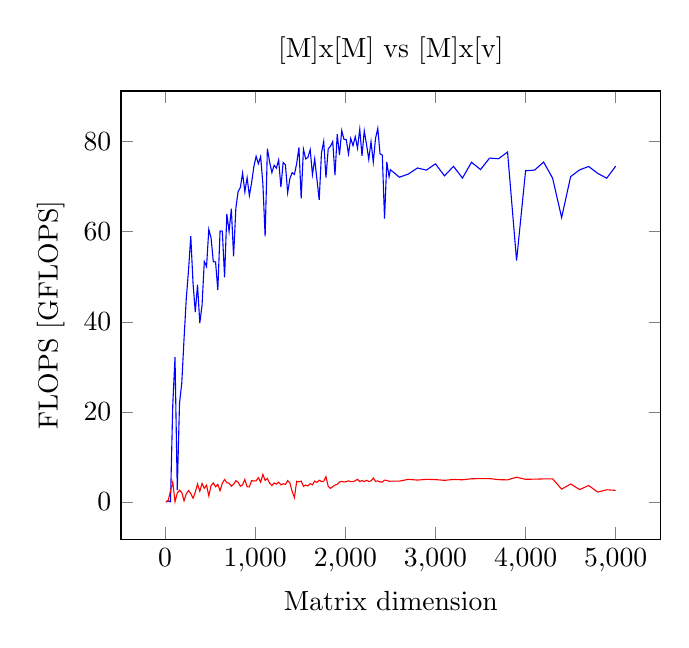
\begin{tikzpicture}
\begin{axis}[xlabel={Matrix dimension}, ylabel={FLOPS [GFLOPS]}, title={[M]x[M] vs [M]x[v]}]
    \addplot[no marks, blue]
        table[row sep={\\}]
        {
            \\
            10.0  0.00023530878984219018  \\
            35.0  0.21910772690106295  \\
            60.0  0.039755514628234866  \\
            85.0  21.442912011173185  \\
            110.0  32.17384998428775  \\
            135.0  2.6431842292559122  \\
            160.0  21.90966009537335  \\
            185.0  26.389082808361486  \\
            210.0  36.12899702143513  \\
            235.0  45.13219325166708  \\
            260.0  51.44069656837638  \\
            285.0  59.01038520070663  \\
            310.0  48.5313211186428  \\
            335.0  42.146549022971016  \\
            360.0  48.21685181864734  \\
            385.0  39.68990730359741  \\
            410.0  43.67801304681091  \\
            435.0  53.37964141365832  \\
            460.0  52.24691358024692  \\
            485.0  60.53778672557497  \\
            510.0  58.6270630913488  \\
            535.0  53.34096946007945  \\
            560.0  53.28932206287961  \\
            585.0  47.03033008821991  \\
            610.0  60.17481584501063  \\
            635.0  60.12283310627119  \\
            660.0  49.89350408776659  \\
            685.0  63.951202008115395  \\
            710.0  60.04144225210726  \\
            735.0  65.09691572575169  \\
            760.0  54.54480277341316  \\
            785.0  65.18104899048775  \\
            810.0  68.92083346274985  \\
            835.0  69.81260005802699  \\
            860.0  73.02857990517683  \\
            885.0  68.8525307065659  \\
            910.0  72.01153413834993  \\
            935.0  68.02836591803735  \\
            960.0  70.89882947566011  \\
            985.0  74.4695339496324  \\
            1010.0  76.74918679872063  \\
            1035.0  75.109105275769  \\
            1060.0  76.67407893120216  \\
            1085.0  70.64983020360992  \\
            1110.0  58.965945890140645  \\
            1135.0  78.44684135836746  \\
            1160.0  75.47563759947788  \\
            1185.0  73.11361687800036  \\
            1210.0  74.75535028279567  \\
            1235.0  74.12810425843301  \\
            1260.0  75.93961885097241  \\
            1285.0  69.90042761391948  \\
            1310.0  75.36300290636987  \\
            1335.0  74.88410098806825  \\
            1360.0  68.65945520969655  \\
            1385.0  71.8209424391753  \\
            1410.0  73.1254485689111  \\
            1435.0  72.71114137952056  \\
            1460.0  75.15012162462537  \\
            1485.0  78.69926205303267  \\
            1510.0  67.40181962053195  \\
            1535.0  78.3220613622165  \\
            1560.0  76.16602502417746  \\
            1585.0  76.52144900985537  \\
            1610.0  78.22227455432987  \\
            1635.0  72.70117362536918  \\
            1660.0  76.1587822842227  \\
            1685.0  71.59822180694208  \\
            1710.0  67.0622776195551  \\
            1735.0  77.449913288636  \\
            1760.0  80.06689767229048  \\
            1785.0  72.00478619294525  \\
            1810.0  78.40867755662231  \\
            1835.0  78.97680511382165  \\
            1860.0  80.02313074654485  \\
            1885.0  72.54850605513857  \\
            1910.0  81.64329243381327  \\
            1935.0  77.03332079636611  \\
            1960.0  82.4523654938911  \\
            1985.0  80.50870958117054  \\
            2010.0  80.44672564698973  \\
            2035.0  77.28083364149391  \\
            2060.0  80.7095771245705  \\
            2085.0  79.12184223578191  \\
            2110.0  81.11313843638882  \\
            2135.0  78.54554270803601  \\
            2160.0  82.77356854110991  \\
            2185.0  76.83335753230769  \\
            2210.0  82.40899230041664  \\
            2235.0  79.40010526534613  \\
            2260.0  76.05476260009156  \\
            2285.0  80.0000075436918  \\
            2310.0  75.4412789245027  \\
            2335.0  80.71820716756916  \\
            2360.0  82.96413544604611  \\
            2385.0  77.30150425497924  \\
            2410.0  77.0084836649049  \\
            2435.0  62.88848610946768  \\
            2460.0  75.50733857314857  \\
            2485.0  72.21697363918317  \\
            2500.0  73.7668990021836  \\
            2600.0  72.10317435866061  \\
            2700.0  72.81326133727134  \\
            2800.0  74.15397428574809  \\
            2900.0  73.67682075984368  \\
            3000.0  75.08242548669931  \\
            3100.0  72.4142201805398  \\
            3200.0  74.51522593104393  \\
            3300.0  71.91374442530405  \\
            3400.0  75.42828453526751  \\
            3500.0  73.8039398913447  \\
            3600.0  76.34734594863151  \\
            3700.0  76.21278837408572  \\
            3800.0  77.70064879000954  \\
            3900.0  53.588442929160415  \\
            4000.0  73.5363431817963  \\
            4100.0  73.68341702367455  \\
            4200.0  75.47356522027998  \\
            4300.0  71.8858956129193  \\
            4400.0  63.14879799442549  \\
            4500.0  72.23636606526392  \\
            4600.0  73.73369762024073  \\
            4700.0  74.4884748659149  \\
            4800.0  72.95570667192224  \\
            4900.0  71.88676217140765  \\
            5000.0  74.56203960930479  \\
        }
        ;
    \addplot[no marks, red]
        table[row sep={\\}]
        {
            \\
            10.0  7.316131887909544e-5  \\
            35.0  0.36616350321327157  \\
            60.0  2.4473147518694764  \\
            85.0  4.39209726443769  \\
            110.0  0.04611667136726402  \\
            135.0  1.951598222412593  \\
            160.0  2.582076756266075  \\
            185.0  2.093912511471398  \\
            210.0  0.25275899916606726  \\
            235.0  1.7858297762255853  \\
            260.0  2.5363950172594927  \\
            285.0  1.857526728031559  \\
            310.0  0.8274603167769516  \\
            335.0  2.1585674305882807  \\
            360.0  3.961848862802641  \\
            385.0  2.376390803860583  \\
            410.0  4.110476702815713  \\
            435.0  3.0352975144967638  \\
            460.0  3.723713154421469  \\
            485.0  1.3351326192949298  \\
            510.0  3.6160909792363247  \\
            535.0  4.199495282949661  \\
            560.0  3.3678422612655186  \\
            585.0  3.903714645845334  \\
            610.0  2.480319421947594  \\
            635.0  4.157494522490011  \\
            660.0  4.9795661741590695  \\
            685.0  4.257302672467371  \\
            710.0  4.160511047101838  \\
            735.0  3.5031661268201586  \\
            760.0  3.9127887087323066  \\
            785.0  4.715309979645869  \\
            810.0  4.382062995912479  \\
            835.0  3.4956681741153353  \\
            860.0  3.7970849312817982  \\
            885.0  4.980319717163495  \\
            910.0  3.3503460190113223  \\
            935.0  3.337182448036952  \\
            960.0  4.721698499877039  \\
            985.0  4.635903194208854  \\
            1010.0  4.694518076724836  \\
            1035.0  5.38936390186475  \\
            1060.0  4.3911809017240735  \\
            1085.0  6.107221693353635  \\
            1110.0  4.790267836662014  \\
            1135.0  5.19785101558276  \\
            1160.0  4.166311888200662  \\
            1185.0  3.648849328488036  \\
            1210.0  4.2132070992295025  \\
            1235.0  3.938437742484826  \\
            1260.0  4.3886176794175045  \\
            1285.0  3.7916963749570884  \\
            1310.0  4.038058127236127  \\
            1335.0  3.8986074409813973  \\
            1360.0  4.731675183392066  \\
            1385.0  4.162923079594086  \\
            1410.0  2.3415361494738876  \\
            1435.0  0.9545409560636974  \\
            1460.0  4.583755793937426  \\
            1485.0  4.4657222442166695  \\
            1510.0  4.636663213046347  \\
            1535.0  3.456951057856587  \\
            1560.0  3.734944196839663  \\
            1585.0  3.5410182898638976  \\
            1610.0  4.058844714466906  \\
            1635.0  3.7814591129667106  \\
            1660.0  4.6291909835266924  \\
            1685.0  4.319668146759707  \\
            1710.0  4.814831280842929  \\
            1735.0  4.519708057691788  \\
            1760.0  4.5697324561500565  \\
            1785.0  5.594363541231376  \\
            1810.0  3.4490709059325155  \\
            1835.0  3.0075679895389715  \\
            1860.0  3.381487635617242  \\
            1885.0  3.7314365436042682  \\
            1910.0  3.8886126358325614  \\
            1935.0  4.426813004400536  \\
            1960.0  4.566353336091023  \\
            1985.0  4.4313841042732856  \\
            2010.0  4.4965542110746055  \\
            2035.0  4.670713420888944  \\
            2060.0  4.5195910896872995  \\
            2085.0  4.506806511775458  \\
            2110.0  4.689459328649246  \\
            2135.0  5.017725743856534  \\
            2160.0  4.535739509960088  \\
            2185.0  4.7396563166544805  \\
            2210.0  4.5126814933491515  \\
            2235.0  4.805147769674967  \\
            2260.0  4.536673277985375  \\
            2285.0  4.65252997705023  \\
            2310.0  5.289633217005218  \\
            2335.0  4.5937690100212825  \\
            2360.0  4.651399737598786  \\
            2385.0  4.429847173202665  \\
            2410.0  4.424605502322725  \\
            2435.0  4.840647980520581  \\
            2460.0  4.760288452273027  \\
            2485.0  4.579449440456163  \\
            2500.0  4.605899014374458  \\
            2600.0  4.618022584589741  \\
            2700.0  5.01807090623676  \\
            2800.0  4.848232992225512  \\
            2900.0  5.011542637442004  \\
            3000.0  4.951175904277266  \\
            3100.0  4.793043752359739  \\
            3200.0  4.9839675886357755  \\
            3300.0  4.911730918331311  \\
            3400.0  5.140655402435274  \\
            3500.0  5.175256360020406  \\
            3600.0  5.183647511969186  \\
            3700.0  4.941519338522229  \\
            3800.0  4.89801179389682  \\
            3900.0  5.48360848117024  \\
            4000.0  5.020353611744365  \\
            4100.0  5.057398159690732  \\
            4200.0  5.1062403380539525  \\
            4300.0  5.129769433648763  \\
            4400.0  2.838174294541066  \\
            4500.0  3.975399638091396  \\
            4600.0  2.7472183278411686  \\
            4700.0  3.6455348592925034  \\
            4800.0  2.188082188697587  \\
            4900.0  2.69516847553144  \\
            5000.0  2.5643789910071333  \\
        }
        ;
\end{axis}
\end{tikzpicture}


      \end{center}
  

\newpage
